\newcommand{\filename}[1]{\colorbox[RGB]{222,222,222}{\mbox{#1}}}
\newcommand{\hltext}[1]{\colorbox[RGB]{237,250,0}{#1}}  % highlight text

\chap{模板使用说明}
\label{chap:模板使用说明}
本章将假定读者已经正确安装 \TeX{} Live 发行版,如果还没有正确安装,请参考第 \ref{chap_tools} 章。

\sect{模板兼容性检查}
\label{sec_check}  % 供后文引用
下载模板后,找到根目录下的 \filename{thesis.tex} 文件,并依次使用 XeLaTeX、Biber、XeLaTeX、XeLaTeX 四次编译\footnote{需要四次编译的原因是存在参考文献引用和各种交叉引用。一次 XeLaTeX 编译不会生成正确的目录和参考文献,并且存在交叉引用的地方会显示为??。}该文件,应当会生成与本文内容相同的 pdf 文档。若运行过程中出现错误,说明存在版本不兼容的问题,或者模板本身有误。此时请检查自己的 \LaTeX 版本是否为 2021 或更新版本,也可自行寻找出错原因并更改模板。

\sect{撰写任务书}

撰写任务书的步骤:

% \begin{varwidth}{\textwidth}
% \begin{enumerate}
  (1)根据第 \ref{sec_check} 节进行模板兼容性检查。

  (2)在文件 \filename{baseinfo.tex} 中填写必要的信息。

  (3)在文件 \filename{task\_book.tex} 中填写任务书内容。

  (4)依次使用 XeLaTeX、Biber、XeLaTeX、XeLaTeX 四次编译文件 \filename{task\_book.tex}。
% \end{enumerate}
% \end{varwidth}

建议每写一部分就编译一次,缩小错误排查范围。

\hltext{该模板任务书后三面尚未制作},若仍要坚持使用该模板,可以在打印时单独打印 word 版任务书的后三面。也可将  word 版任务书的后三面导出为 pdf ,并在\href{https://www.ilovepdf.com/zh-cn/merge_pdf}{这个网站}合并 pdf。

\sect{撰写开题报告}

撰写开题报告的步骤:

(1)根据第 \ref{sec_check} 节进行模板兼容性检查。

(2)在文件 \filename{baseinfo.tex} 中填写必要的信息。

(3)在文件 \filename{researchProposal.tex} 中填写开题报告内容。

(4)依次使用 XeLaTeX、Biber、XeLaTeX、XeLaTeX 四次编译文件 \filename{researchProposal.tex}。

建议每写一部分就编译一次,缩小错误排查范围。

\sect{撰写外文译文及原文}

撰写外文译文及原文的步骤:

(1)根据第 \ref{sec_check} 节进行模板兼容性检查。

(2)在文件 \filename{baseinfo.tex} 中填写必要的信息。

(3)在文件 \filename{translation.tex} 中填写内容。

(4)依次使用 XeLaTeX、Biber、XeLaTeX、XeLaTeX 四次编译文件 \filename{translation.tex};若没有目录、参考文献和交叉引用,使用一次 XeLaTeX 编译即可。

建议每写一部分就编译一次,缩小错误排查范围。


\sect{撰写论文正文}

撰写论文正文的步骤:

(1)根据第 \ref{sec_check} 节进行模板兼容性检查。

(2)在文件 \filename{baseinfo.tex} 中填写必要的信息。

(3)在文件 \filename{thesis.tex} 中填写正文内容。

(4)依次使用 XeLaTeX、Biber、XeLaTeX、XeLaTeX 四次编译文件 \filename{thesis.tex}。

建议每写一部分就编译一次,缩小错误排查范围。

由于正文内容较多,因此\textbf{强烈建议}将不同章节的内容写入多个 tex 文件,并用 \verb!\include! 命令导入。


\sect{插入图片}

相信初次看到本文的大部分同学还在以最原始的方式手动调整图片编号及位置。 \LaTeX{} 也可以对图片手动编号,然而通过这种方式管理的图片难以维护:只要稍微对文章内容调整一下,就可能要改动一大批图片的编号。不仅如此,word 还容易出现图片与图题不在同一面的情况。

本模板使用 \verb!\figure! 环境管理图片。figure是一种浮动体,它可以在文字间自由浮动以调整图片的位置、自动编号。

使用 \verb!\includegraphics! 命令即可在本模板中插入图片,为了对图片进行编号及引用,应将其放入 figure 环境。插入图片代码示例:

\begin{lstlisting}[numbers=none,language=TeX]
长沙理工大学校徽如图 \ref{fig.csustlogo} 所示。  % 使用 \ref 命令引用图片标签

\begin{figure}[htbp]  % htbp 选项允许浮动体出现在任意位置,后文详述
  \centering  % 表格居中
  
\includegraphics[scale=.5]{figure/template/csustlogo_626by572.jpg}  % 选项代表缩小到原图的 0.5 倍。
  \caption{长沙理工大学校徽}  % 图题
  \label{fig.csustlogo}  % 定义标签,方便引用该图
\end{figure}
\end{lstlisting}

长沙理工大学校徽如图 \ref{fig.csustlogo} 所示。  % 使用 \ref 命令引用图片标签

\begin{figure}[htbp]  % htbp选项允许浮动体出现在任意位置,后文详述
  \centering  % 表格居中
  
\includegraphics[scale=.5]{figure/template/csustlogo_626by572.jpg}  % 选项代表缩小到原图的 0.5 倍。
  \caption{长沙理工大学校徽}  % 图题
  \label{fig.csustlogo}  % 定义标签,方便引用该图
\end{figure}

关于 \verb!\includegraphics! 命令与 figure 环境的更多用法可以参考 \href{https://zhuanlan.zhihu.com/p/262389031}{\LaTeX{}插图总结} 。

\sect{绘制表格}

相信初次看到本文的大部分同学还在以最原始的方式手动调整表格编号及位置。 \LaTeX{} 也可以对表格手动编号,然而通过这种方式管理的表格难以维护:只要稍微对文章内容调整一下,就可能要改动一大批表格的编号。不仅如此,word 还容易出现表格与表题不在同一面的情况。

本模板使用 \verb!\table! 环境管理表格。table也是一种浮动体,它可以在文字间自由浮动以调整表格的位置、自动编号。

使用 tabular 环境即可在本模板中绘制表格,为了对表格进行编号及引用,应将其放入 table 环境。插入表格代码示例:

前面提到的figure和table都是浮动体,我们可以为浮动体环境添加选项来指定它们允许浮动的位置,浮动体选项及其含义如表 \ref{标签名都可以随便取} 所示。关于浮动体选项和位置更详细的说明参见\href{https://www.latexstudio.net/archives/10043.html}{浮动算法}。

\begin{table}[htbp]
  \centering  % 表格居中
  \zihao{5}  % 五号字体
  \caption{浮动体选项及其含义}
  % \vspace{-3mm}
  \begin{tabular}[]{ll}
      \toprule   % 三线表的第一条线
      表项      & 含义            \\
      \midrule   % 三线表的第二条线
        !       &  忽略一些严格的限制   \\
        h       &  如果可以,放在当前位置   \\
        t       &  允许放在顶部   \\
        b       &  允许放在底部  \\
        p       &  运行放在浮动栏或浮动页   \\
        H       &  禁止浮动   \\
      \bottomrule   % 三线表的第三条线
  \end{tabular}
  \label{标签名都可以随便取}  % 注意:这不是伪代码
\end{table}

绘制表 \ref{标签名都可以随便取} 的代码如图 \ref{fig.tablecode} 所示。

\begin{figure}[htbp]
  \centering
  \begin{minipage}{8cm}
  \begin{lstlisting}[language=TeX]
\begin{table}[htbp]
  \centering  % 表格居中
  \zihao{5}  % 五号字体
  \caption{浮动体选项及其含义}
  % \vspace{-3mm}  % 适当调整标题与表的间距
  \begin{tabular}[]{ll}  % 两列、左对齐
      \toprule   % 三线表的第一条线
      表项      & 含义            \\
      \midrule   % 三线表的第二条线
        !       &  忽略一些严格的限制   \\
        h       &  如果可以,放在当前位置   \\
        t       &  允许放在顶部   \\
        b       &  允许放在底部  \\
        p       &  运行放在浮动栏或浮动页   \\
        H       &  禁止浮动   \\
      \bottomrule   % 三线表的第三条线
  \end{tabular}
  \label{标签名都可以随便取}  % 注意:这不是伪代码
\end{table}
  \end{lstlisting}
  \end{minipage}
  \caption{绘制表 \ref{标签名都可以随便取} 的代码}
  \label{fig.tablecode}
\end{figure}

关于 tabular 环境的更多用法可以参考 \href{https://zhuanlan.zhihu.com/p/19749566}{\LaTeX{}下的表格处理}。

\sect{使用公式}

排版数学公式是 \TeX{} 系统设计的初衷,它在 \LaTeX{} 中占有特殊的地位,也是 \LaTeX{} 最为人所称道的功能之一\cite{lhy_latex}。

\LaTeX{} 的数学公式包括行内公式和行间公式两种,行内公式由美元符号包裹,形如 \verb!$...$! ,行间公式由 \verb!\[! 和 \verb!\]! 包裹。

下面以 $Fibonacci$ 数列的通项公式为例展示 \LaTeX{} 数学公式的效果。

$Fibonacci$  数列的通项公式为:

\[
  F_n=\dfrac{1}{\sqrt{5}}\left( \dfrac{1+\sqrt{5}}{2}\right) ^{n}-\dfrac{1}{\sqrt{5}}\left( \dfrac{1-\sqrt{5}}{2}\right) ^{n}.(n\in \mathrm{N})​​​​​
\]

由于

\[
\left| F_{n}-\dfrac{1}{\sqrt{5}}\left( \dfrac{1+\sqrt{5}}{2}\right) ^{n}\right| =\dfrac{1}{\sqrt{5}}\left( \dfrac{\sqrt{5}-1}{2}\right) ^{n}\le \dfrac{1}{\sqrt{5}} <\dfrac 12.(n\ge 0)
\]

因此通项公式可化为:

\[
F_{n}=\left\lfloor \dfrac{1}{\sqrt{5}}\left( \dfrac{\sqrt{5}+1}{2}\right) ^{n}+\dfrac{1}{2}\right\rfloor.(n\ge 0)
\]

关于 \LaTeX{} 公式更详细的介绍参见 \href{https://zhuanlan.zhihu.com/p/110756681}{\LaTeX{}公式篇}。

\sect{交叉引用}

用 \verb!\label! 命令在适当的位置定义标签后,即可用 \verb!\ref! 命令引用,如:本文第 \ref{chap:模板使用说明} 章的内容在第 \pageref{chap:模板使用说明} - \pageref{chap:模板使用说明:end} 页。

前面图和表的引用就是用的这种方法。标签的命名可以为任意不含特殊字符的字符串,建议图标签使用 \verb!fig:有意义的字符串! 、表标签使用 \verb!tab:有意义的字符串! ,方便记忆。

\hltext{本文源码中的标签命名并没有规范化,请勿模仿。}

\sout{\xout{因为作者本人写到这里时才发现有这么好用的命名方法}。}

\sect{管理参考文献}

相信初次看到本文的大部分同学还在以最原始的方式手动调整参考文献。 \LaTeX{} 也可以通过上标命令 \verb!$^\text{[编号]}$! 的方式手动引用,效果就像这样 $^\text{[编号]}$ 。然而通过这种方式管理的参考文献难以维护:只要稍微对文献调整一下,整个顺序编号都要重新变动。

因此推荐使用 BibLaTeX 自动管理参考文献的引用和列表,biblatex 宏包已经引入,在 \filename{reference.bib} 文件中导入参考文献条目后,正文中直接引用即可。引用参考文献的命令包括 \verb!\cite! 和 \verb!\parencite! , 效果就像这样 \cite{sample} 和这样\parencite{sample},点击编号可以跳转到对应的参考文献条目。

不知道如何使用 BibLaTeX 管理参考文献的同学可以参考这篇教程 \href{https://www.overleaf.com/learn/latex/Bibliography_management_with_biblatex}{Bibliography management with biblatex}。

可以手动在 bib 文件中添加参考文献条目,但还是推荐使用 \href{https://www.jabref.org/}{JabRef} 或者其他工具进行可视化添加,避免 bib 文件的编译错误。


\sect{辅助工具}
\subsect{字数统计}
使用 \LaTeX 写论文同样可以进行字数统计,只是不如 word 简单直观。

在 \filename{thesis.tex} 所在文件夹下打开命令行窗口,在命令行输入 

\begin{quote}
texcount thesis.tex body/*.tex
\end{quote}

回车即可显示字数统计信息。本文的字数统计信息如图 \ref{fig:specification:texcount} 所示。

\begin{figure}[htbp]  % htbp 选项允许浮动体出现在任意位置,后文详述
  \centering  % 表格居中
  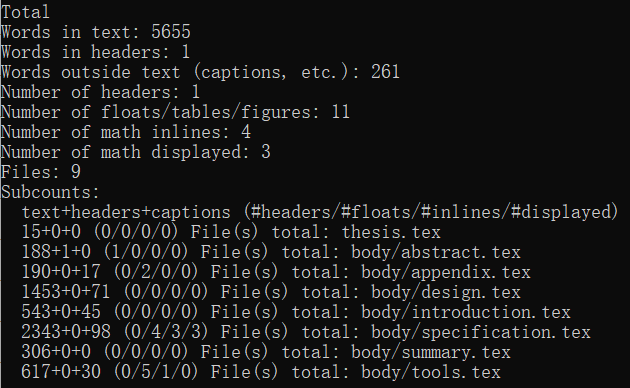
\includegraphics[scale=.5]{figure/thesis/texcount.png}  % 选项代表缩小到原图的 0.5 倍。
  \caption{本文字数统计信息}  % 图题
  \label{fig:specification:texcount}  % 定义标签,方便引用该图
\end{figure}

\subsect{pdf 的拆分与合并}
如果最后需要将论文正文、任务书、开题报告、外文译文及原文并入一个 pdf ,可能需要对 pdf 进行拆分与合并。

\LaTeX{} 本身具有合并拆分 pdf 的功能\footnote{使用 pdfpages 宏包。},但是需要自己查文献写代码,相对来说比较麻烦,因此我们可以使用工具对 pdf 进行拆分与合并。

很多浏览器(比如 Edge)和 pdf 阅读器(比如Adobe )应该都具有打印指定页面 pdf 的功能,多次打印不同页面即可达到拆分 pdf 的目的。\hltext{推荐使用谷歌浏览器的打印功能},用谷歌浏览器打开 pdf 就能看到打印按钮了。

\href{https://www.ilovepdf.com/zh-cn/merge_pdf}{ilovepdf 这个网站}可以免费合并多个pdf文件,比较方便。

\subsect{pdf 转 word}
由于学校要求提交 word 稿查重,并且毕业答辩后还要同时提交论文的 word 版和 pdf 版。因此我们使用 \LaTeX{} 编排好精美的pdf论文后,还要将其转成 word 。

好在使用 \LaTeX{} 撰写的 pdf 文件可以\href{https://www.pdfwordconvert.com/zh/convertform}{在这里}轻松转成 word ,并且可以保留几乎所有格式。根据本人亲测的结果,转换后的 word 只存在参考文献引用位置有一点偏差、代码边框展示不全的问题。

转换拆分合并后的 pdf 文件时可能会失败,遇到这种情况时可先将 \LaTeX{} 直接生成的 pdf 文件转成 word ,需要的话再设法合并 word 吧。

打印时使用 pdf 版本即可,甘饴后面的未来图文打印pdf比word每张便宜5分钱(2022年如此,图书馆不清楚)。


\label{chap:模板使用说明:end}

\let\filename\undefined
\let\hltext\undefined
